\section{GUI Implementation}

\subsection*{Application Architecture}

The GUI is built using the Flet framework, creating a responsive web based interface that runs in the browser. The application follows a two panel layout design where the main game display occupies the left panel and the multimodal input controls are positioned on the right panel.

To launch the application, use the following command from the project root:

\begin{lstlisting}[caption={Starting the Frontend Application}]
flet run frontend/main.py --web
\end{lstlisting}

This opens the game in the default web browser as a responsive web application.

\subsection*{Main Components}

The interface is organized into modular components, each handling specific aspects of the game:

\begin{center}
\begin{tabularx}{\linewidth}{@{}lX@{}}
\toprule
\textbf{Component} & \textbf{Responsibility} \\ \midrule
\texttt{GamePanel}        & Main game interface with word display, hangman visual, and control buttons. \\
\texttt{GameDisplay}      & Shows current word state, guessed letters, remaining attempts, and game status. \\
\texttt{HangmanVisual}    & Animated hangman drawing that progresses with wrong guesses (7 states). \\
\texttt{MediaControls}    & Tabbed interface for voice input, hand drawing, and AI agent chat. \\
\texttt{ManualInput}      & Text input field for manual letter guessing with validation. \\
\texttt{AppLayout}        & Responsive layout manager handling window resizing and notifications. \\ \bottomrule
\end{tabularx}
\end{center}

\subsection*{Game Panel Layout}

The left panel contains the core game interface:

\begin{itemize}
\item \textbf{Control Buttons}: Three action buttons for starting new games, resetting, and revealing words
\item \textbf{Word Display}: Shows the target word with revealed letters or underscores for hidden letters
\item \textbf{Game Information}: Displays guessed letters, remaining attempts, and current game status
\item \textbf{Hangman Visual}: Animated SVG style drawing showing game progress (0-6 wrong guesses)
\item \textbf{Manual Input}: Text field for direct letter input with real time validation
\end{itemize}

\subsection*{Multimodal Input Interface}

The right panel provides three input modalities through a tabbed navigation interface:

\begin{description}
\item[\textbf{Agent Chat}] Natural language conversation with an AI agent that manages the game, processes letter guesses, and provides guidance. Includes voice to text capability for hands free interaction.

\item[\textbf{Voice Input}] Direct voice recognition for letter guessing. Users say "Letter X" to guess a specific letter, with visual feedback showing the recognized input and confidence levels.

\item[\textbf{Hand Drawing}] Computer vision based letter recognition using webcam input. Users draw letters in the air, which are captured, processed through a CNN model, and converted to game guesses.
\end{description}

\subsection*{State Management and Observer Pattern}

The application uses a centralized state management system with an observer pattern for real time UI updates:

\begin{lstlisting}[style=pystyle, caption={Observer Pattern Implementation}]
class GameStateManager:
    def add_observer(self, callback: Callable[[GameState], None]) -> None:
        """Add a callback function to be called when game state changes"""
        if callback not in self._observers:
            self._observers.append(callback)
    
    def _notify_observers(self, state: GameState) -> None:
        """Notify all observers of a state change"""
        for callback in self._observers:
            callback(state)

# Components register as observers
self.state_manager.add_observer(self.on_state_changed)
\end{lstlisting}

This ensures that all UI components automatically update when the game state changes, whether triggered by manual input, voice commands, hand gestures, or AI agent actions.

\newpage
\subsection*{Component Implementation Details}
\subsubsection*{GameDisplay Component}
The \texttt{GameDisplay} component handles the visual representation of the current game state:

\begin{figure}
    \centering
    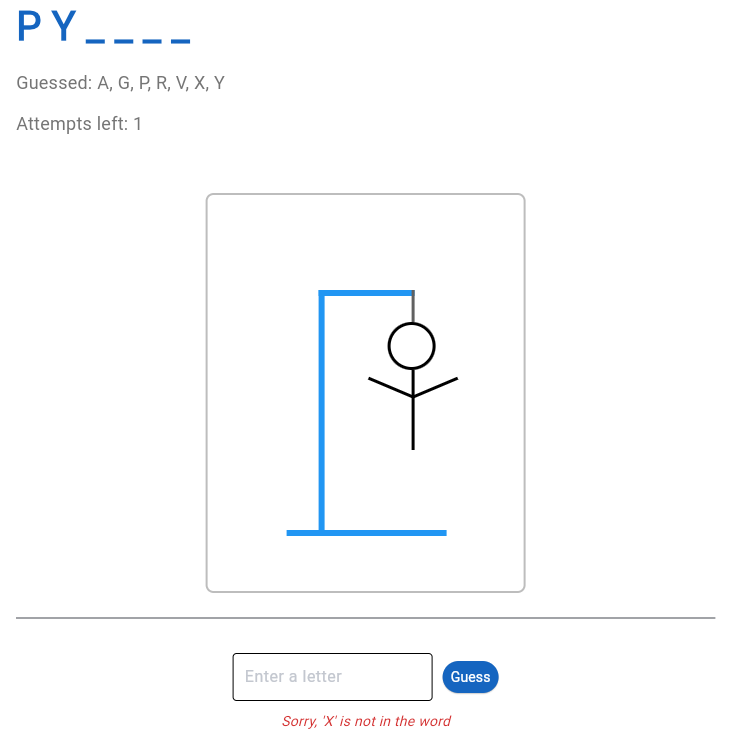
\includegraphics[width=0.55\textwidth]{./images/hang-man.png}
    \caption{GameDisplay component showing the current word state, guessed letters, and remaining attempts.}
\end{figure}

\subsubsection*{HangmanVisual Component}

The hangman visual progresses through seven distinct states, from an empty gallows to a complete figure:

\begin{lstlisting}[style=pystyle, caption={Hangman Visual State Management}]
def update_state(self, wrong_guesses):
    """Update the hangman visual based on number of wrong guesses"""
    wrong_guesses = max(0, min(wrong_guesses, 6))
    self.current_state = wrong_guesses
    self.content = self.states[wrong_guesses]
    self.update()
\end{lstlisting}

\subsubsection*{MediaControls Navigation}

The multimodal interface uses a navigation bar to switch between input methods:
